
\documentclass[runningheads,a4paper]{llncs}

\usepackage{amssymb}
\setcounter{tocdepth}{3}
\usepackage{graphicx}

\usepackage{url}
\urldef{\mailsa}\path|{ismael.rivera, knud.moeller}@deri.org| 
\urldef{\mailsb}\path|zuendorf@cs.uni-kassel.de|
%\urldef{\mailsc}\path|erika.siebert-cole, peter.strasser, lncs}@springer.com|    
\newcommand{\keywords}[1]{\par\addvspace\baselineskip
\noindent\keywordname\enspace\ignorespaces#1}

\usepackage{amssymb}

\newenvironment{listing}
{\begin{list}{}{\setlength{\leftmargin}{1em}}\item\scriptsize\bfseries}
{\end{list}}

\begin{document}

\mainmatter  % start of an individual contribution

% first the title is needed
\title{Web Service Wrapping, Discovery and Consumption --- More Power to the End-User}

% a short form should be given in case it is too long for the running head
\titlerunning{Web Service Wrapping, Discovery and Consumption --- More Power to the End-User}

% the name(s) of the author(s) follow(s) next
%
% NB: Chinese authors should write their first names(s) in front of
% their surnames. This ensures that the names appear correctly in
% the running heads and the author index.
%
\author{Ismael Rivera\and Knud M\"oller\and Albert Z\"undorf}
%
\authorrunning{Ismael Rivera\and Knud M\"oller\and Albert Z\"undorf}
% (feature abused for this document to repeat the title also on left hand pages)

% the affiliations are given next; don't give your e-mail address
% unless you accept that it will be published
\institute{DERI, National University of Ireland, Galway\\
University of Kassel, Germany\\
\mailsa\\
\mailsb\\
%\mailsc\\
%\url{http://www.springer.com/lncs}
}

%
% NB: a more complex sample for affiliations and the mapping to the
% corresponding authors can be found in the file "llncs.dem"
% (search for the string "\mainmatter" where a contribution starts).
% "llncs.dem" accompanies the document class "llncs.cls".
%

\toctitle{Lecture Notes in Computer Science}
\tocauthor{Authors' Instructions}
\maketitle


%!TEX root = paper.tex

\begin{abstract}
B2B systems integration was revolutionised by the introduction of web services. The way enterprise systems communicated was dramatically transformed, and by adopting these technologies, the relationships with providers and customers were strengthened. The main advantages seen by companies which adopted the technology were an increase of operational efficiencies, and reduction of costs. 
In this scenario, highly qualified software developers are responsible for the integration of services with other systems, by means of the analysis of WSDL service description or human-readable specifications. 
However this model fails when it tries to target the long tail of enterprise software demand, and as a result, the end-users. Discovery and consumption of web services is far from a straight-forward task for an end-user, meaning potential users, willing to create their task-specific applications, have been ruled out. 
This paper presents an approach to facilitate the discovery and consumption of web services by end-users on the Internet, closing the gap between business web services and the latter. The process includes: (a) a way to generate ready-to-use web services wrappers, and (b) a catalogue which users can browse to search for web services fitting their needs. These web services wrappers are described by a model created, although highly influenced by well-known web services modelling standards. Furthermore, two prototypes have been developed to serve as a proof of concept.
\keywords{web services, end-users, discovery, consumption, linked data}
\end{abstract}


%!TEX root = paper.tex

\section{Introduction}
\label{sec:introduction}

Business-to-business (B2B) integration is still a significant challenge, often requiring extensive efforts in terms of different aspects and technologies for protocols, architectures or security. Solutions based on open standards have reduced the complexity of integrating different business applications between different companies and partners. 
In this sense, Web services and XML standards such as RosettaNet, ebXML or OAG have been a boon to the world of B2B. By web services standards we are referring to the following open standards: Web Services Description Language (WSDL --- to describe), Universal Description, Discovery and Integration (UDDI --- to advertise and syndicate), Simple Object Access Protocol (SOAP --- to communicate) and Web Services Flow Language (WSFL --- to define work flows). 
A common scenario  in their usage is a company using WSDL to describe its web services, publishing them through a repository using UDDI, while these web services use SOAP-based messages to achieve dynamic integration between different, disparate applications.

While the adoption of these standards has offered some advantages in business-to-consumer (B2C) integration as well,  the interaction and consumption of web services still requires programming skills and a deep understanding of the  technology, which poses an obstacle for an end-user with limited knowledge on the matter (in the sense as defined in~\cite{fuchsloch2010}). 
Regarding the discovery of the right service for the right task --- a crucial requirement for the dynamic use of WS --- most publishing platforms are syntax-based, %leading to poor precision and recall in finding the correct service, 
making it difficult to navigate through a large number of web services~\cite{pilioura_acm2009}, 
therefore preventing end-users from performing these tasks. 
Solutions such as Semantic Web Services (SWS) promised many advantages in discovery, composition and consumption of web services, independently of the provider's platform, location, service implementation or data format. 
However, as of yet they have not been widely adopted, 
possibly because the perceived potential benefits of SWS did not justify the additional investments required for businesses~\cite{shi2007}.
In a similar vein as B2C, governments are currently opening their data to the public as linked data. 
So far, the efforts are restricted to data only, so that users are left alone in finding applications of that data. 
A natural further development in the public sector would be that their services for administration tasks and single-window applications will be opened as well. Hence, governments will benefit from the research done around these concepts and technologies.

The motivation of our work has been strongly influenced by the end-users' needs. We are targeting users which are non-skilled in term of programming and software development, empowering them with a platform to discover and consume web services in a straight-forward manner.
The web services and their specifications are not published right away in the platform, since this would simply mean to reimplement UDDI.
However, their definition and behaviour are wrapped in what we call a ``web service wrapper''. The products resulting from the wrapping process are two artifacts: a specific definition of the web service to be used by this tool, and a ready-to-consume (inside a web browser) piece of code with the proper functions to invoke the web service.

The remainder of this paper is organised as follows. Section~\ref{sec:related_work} covers the state of the art in web services publication, discovery and wrapping/consumption. In Section~\ref{sec:wrapping_web_services} we present our approach for web services wrapping, available possibilities and limitations. Next, Section~\ref{sec:discovery} describes our platform for publishing web services and empowering end-users to discover services. Section~\ref{sec:use_case} gives the reader a clearer use case and how this work is integrated into the FAST platform, and finally, we present our main conclusions and highlight future lines of research in Section~\ref{sec:conclusions}.




\section{Related work}
\label{sec:related_work}

Web services have been around for a long time since they first appeared. One of their most important claims has been (syntactic) interoperability between third-party systems and applications based on different platforms / programming languages. System integration, within a company or between systems from different enterprises became easier with the adoption of the web services standard technologies, being the Web Service Description or WSDL the most extended standard used for the definition of web services. Many integrated development environments (IDEs) can deal with WSDL to facilitate the integration task, however it is still required that developers read and understand their specifications, and implement part of the logic in a programmatically-fashion way. A step forward, there are several tools which facilitate the interaction with data sources and services on the Web. Yahoo! Pipes, Apatar, JackBe Presto, Microsoft Popfly and NetVibes, among others provide a set of modules to access different kind of data sources, such as RSS feeds, a given web page (HTML code), Flickr images, Google base or the Yahoo! search engine, databases (MySQL, PostgreSql, Oracle), and powerful enterprise systems such as Salesforce CRM, SugarCRM and Goldmine CRM. However, none of the solutions in the market really facilitate end-users to build up their own applications or widgets allowing the interaction with Web services created by third-party providers. The solutions found are mainly data-oriented (RSS feeds, databases, raw text). Several tools permits some sort of (Web) service integration, but are meant to be used within an entreprise level by savvy business users or developers. [TODO: rewrite this paragraph] This paper presents an approach to leverage the possibility of integrate REST or SOAP-based web service inside a widget or any application for a web browser (by creating service wrappers), and graphical tool will be provided to facilitate the process of building these service wrappers.

In the context of publishing and discovering Web services, a service provider have well-known and widely used technologies to accomplish the task of publication, such as the Universal Description, Discovery and Integration (UDDI) or WS-Discovery. The UDDI service registry specification \cite{uddi2004} is currently one of the core standards in the Web service technology stack and an integral part of every major SOA vendor's technology strategy and offers to requesters the ability to discover services via the Internet. In a few words, UDDI serves as a centralised repository of WSDL documents. A similar concept is iServe \cite{pedrinaci_ores2010}. This platform aims to publish Web services as what they called Lined Services Linked Services --linked data describing services, storing Web service definitions in a semantic-annotation fashion so semantic Web technologies for Web service discovery and processing can make use of them. However, the platform does not deal with the step from the definition to the consumption of the services.

A different approach for Web service discovery is the Web Services Dynamic Discovery (WS-Discovery) specification. The core of this approach is a multicast discovery protocol. Service providers and consumers  listen each other for new services specifications within a network, so there is no need of a centralised registry. As a drawback, WS-Discovery do not support Internet-scale discovery, therefore make if useless for our purposes.



\section{Wrapping web services}
\label{sec:wrapping_web_services}

In our approach, wrapping web services is done in two steps: a first step is in charge of the construction of a service request and a second step analyzes the response got from the execution of the service, allowing the analysis of response data and the mapping to domain-specific concepts. From this input, we generate JavaScript code to be embedded into web gadgets. This JavaScript code takes query parameters, constructs the service request, analysis the service response and returns result data in the desired format. 

\subsection{Constructing service requests} % (fold)
\label{sub:constructing_service_requests}

As a first approach, the interaction with services is limited to simple GET requests as supported e.g. by REST services. Support for other services like SOAP services is planned. A service request is thus assembled using a certain URL and a set of parameters. As an example, the Ebay Shopping web service will be studied. The following URL is invoked to retrieve a list of items corresponding to the search keywords \emph{USB}:

\begin{listing}
\begin{verbatim}
http://open.api.sandbox.ebay.com/shopping?appid=KasselUn-efea-4b93-9505-5dc2ef1ceecd
  &version=517&callname=FindItems&ItemSort=EndTime&QueryKeywords=USB&responseencoding=XML
\end{verbatim}
\end{listing}

As you may see, the URL invoked is \url{http://open.api.sandbox.ebay.com/shopping} and the parameters used in the example are:
\begin{description}
	\item[appid] this is the application ID obtained to use the API.
	\item[version] the API version.
	\item[callname] in this case FindItems to search through all items in Ebay.
	\item[itemsort] sorting method for the list of items.
	\item[querykeywords] list of keywords.
	\item[responseencoding] format of the response message obtained by the invocation of the request.
\end{description}

The above URL for searching items in Ebay is followed by the query parameters, which take the form \textit{argument=value}. In this example, the only relevant parameter the end user may want to provide is \emph{querykeywords}. Thus the end user may use some input field to provide a query keyword and pass this value to our service wrapper operation. Other parameters can be set to a default value. However, in order to develop a more generic wrapper to a service, more or even all parameters might be passed by the user.

To define the desired input parameters and the type of the expected result of a new service wrapper the FAST service wrapper tool provides a web based form that allows the editing of these entries, cf. Figure \ref{fig:construct_pre_post_conditions}. Note, we allow to edit example values for the input parameters. These example values may be used to test the service wrapper. 

\begin{figure}
  \begin{center} 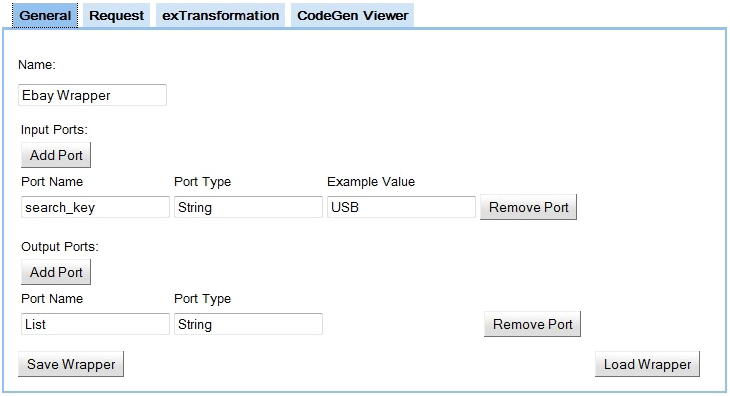
\includegraphics[width=\linewidth]{images/ServiceWrapperToolGVSWithPortDefinitions.png}
    \caption{Configuring parameters of a service wrapper}
    \label{fig:construct_pre_post_conditions}
  \end{center}
\end{figure}

The service wrapper tool composes the request using a template string which will contain placeholders for input values. Before sending the request to the service, the placeholders are replaced with their corresponding values and the resulting URL is then ready to be sent as the service request.

An example of service request construction can be found in the Figure~\ref{fig:construct_service_request}. In the top input field the user may drop an example HTTP request taken e.g. form the service documentation e.g. from its website\footnote{http://developer.ebay.com/products/shopping/}. The tool analyses the example request and in the middle of the screen a form for editing the request parameters is provided. In our example, the user has connected the \textit{QueryKeywords} parameter with the input parameter \textit{search\_key} by adding a corresponding reference to the value field of that parameter. In addition, we have retrieved an access key which has been entered as value for the \textit{appid} parameter.

\begin{figure}
  \begin{center}
    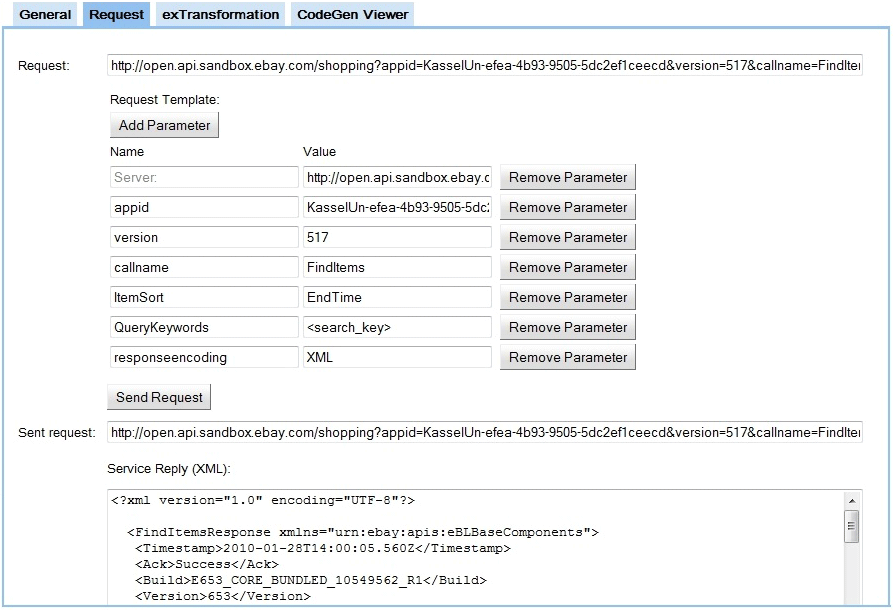
\includegraphics[width=\linewidth]{images/ServiceWrapperToolGVSWithRequestExample.png}
    \caption{Constructing the service request URL and its parameters}
    \label{fig:construct_service_request}
  \end{center}
\end{figure}

Below the request parameter editing form of Figure ~\ref{fig:construct_service_request}, a \textit{Send Request} button allows to validate the constructed URL by sending it to the specified service address (via a server relay). Then the placeholders for input parameters are replaced by their example values and the resulting http request is shown below the parameter form. In addition, the request is send and the response is shown on the bottom of that page. This gives the user a fast feedback whether the constructed request works as desired. 

\subsubsection{Limitations} % (fold)
\label{ssub:limitations}



It is worth pointing out that currently the wrapper tool is able to construct input ports for the wrappers using just basic types. To construct URL requests from more complex input parameters, as e.g. a person object, we are currently developing access operations that will allow to access the values of fields of complex objects. For example, the expression \emph{customer.address} may refer to the \emph{address} field of a \emph{customer} parameter.  

% subsubsection limitations (end)

% subsection constructing_service_requests (end)

\subsection{Interpreting service responses} % (fold)
\label{sub:interpreting_service_responses}

Once the service request is constructed and sent to the service provider, it will send back a response. This response message could be serialized in any format, though the most common formats used nowadays are XML or JSON among others. To continue the example started in the previous section, the response of the Ebay Shopping service will be in XML as specified in the request.

\subsubsection{Translation XML into Facts} % (fold)
\label{ssub:translation_xml_into_facts}

Figure ~\ref{fig:response_service_execution} shows the data transformation tab of the wrapper tool. 

\begin{figure}
  \begin{center}
    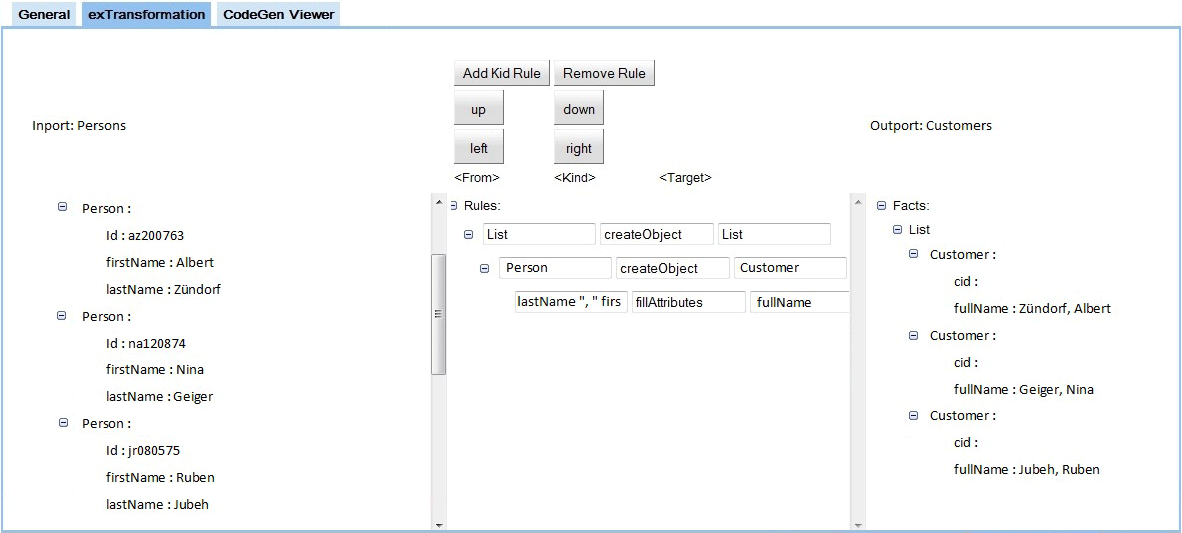
\includegraphics[width=\linewidth]{images/ServiceWrapperToolGVSWithTransformationRules.png}
    \caption{Interactive, rule based transforming of an XML response to domain objects}
    \label{fig:response_service_execution}
  \end{center}
\end{figure}

Once the service response, in XML format, has been retrieved, the transformation tab shows it as an interactive object tree on the left side of Figure ~\ref{fig:response_service_execution}. To construct this interactive object tree, the XML document has been parsed into a DOM, and a simplified tree representation of that DOM is built up. 

A transformation rule is used to analyze the XML data and to generate domain-specific objects from concepts from the ontologies used by the parameters of the different building blocks. A transformation rule is composed of three elements, cf. the middle part of Figure ~\ref{fig:response_service_execution}. First, the \textit{from} field indicates the XML elements to be translated by the rule. These XML elements are identified by the tag name of a DOM element from the XML document. Second, the type of the rule will be set, taking one of the following values: \emph{createObject}, \emph{fillAttributes} or \emph{dummy}. And third, the target of the rule specifies a certain concept or attribute, to be created or filled. A detailed explanation of the type of actions to be trigger from the transformation rules is:
\begin{description}
	\item[action \emph{createObject}] specifies the creation of a new domain object. The type of that new object is provided in the third compartment. In the example being explained, the root rule searches for XML elements with tag name \emph{FindItemsResponse} and for each such element a \emph{List} object is created. The resulting objects are shown in a facts tree in the right of Figure ~\ref{fig:response_service_execution}.
	\item[action \emph{fillAttributes}] does not create a new object but it fills the value of the attribute provided as third part of such rules. In our example, the third transformation rule searches for XML elements with tag name \emph{Title}. Note, the rule is a sub-rule of the second rule, which generates \emph{Product} objects. Thus, the sub-rule searches for \emph{Title} tags only in the subtree of the XML data that has been identified by an application of the parent rule before. For example, the \emph{Item} rule may just have been applied to the first \emph{Item} element of the XML data. Then, the \emph{Title} rule is applied only to the first \emph{Item} sub-tree of the XML data and thus it will find only one \emph{Title} element in that sub-tree (not visible in Figure ~\ref{fig:response_service_execution} ). The value of that \emph{Title} element is then transfered to the \emph{productName} attribute of the corresponding \emph{Product} object. Actually, our \textit{from} fields allows also to refer to parts of an XML attribute e.g. to \textit{words} 1 through 3. It is also possible to combine constant text and elements of multiple XML tree elements. 
	\item[action \emph{dummy}] does not create or modify any objects but such rules are just used to narrow the search space for their sub-rules. For example, in Amazon product data, the XML data for an item contains sections for \emph{minimum price}, \emph{maximum price}, and \emph{average price}. Each such section contains the \emph{plain price} and the \emph{formatted price}. Thus, in the Amazon case, a rule that searches for \emph{formatted price} elements within an \emph{Item} element would retrieve three matches. Using a dummy rule, we may first search for \emph{minimum price} elements and then search for \emph{formatted price} elements within that sub-tree.
\end{description}

Our tool follows an interactive paradigm. Therefore, any time a change to a transformation rule is done, the transformation process is triggered and the resulting facts tree is directly shown. This process helps the user to deal with the slightly complex semantics of the transformation rules avoiding errors or mistakes. In addition, out tool is ontology-driven, therefore, the service wrapper designer shall retrieve the domain-specific types from a FAST ontology server together with the structure of each type, i.e. together with a description of the attributes of each object. Thus, the transformation rule editor is able to provide selection boxes for the target element of the rules. For a \emph{createObject} rule, this selection box shows the object types available for that domain. For the \emph{fillAttributes} rules, the selection box shows the attributes of the object type chosen in the parent rule. In addition, we may provide some analysis tool, which will help to guarantee that the objects generated by the transformation rules conform to the object types defined in the corresponding FAST ontology. This helps to ensure that the objects generated by the designed service wrapper will be compatible for input parameters of subsequent filter steps and or gadgets.

% subsubsection translation_xml_into_facts (end)

% subsection interpreting_service_responses (end)

\subsection{Generating a Resource Adapter} % (fold)
\label{sub:generating_a_resource_adapter}

Once the wrapping of a service has been defined and tested in the service wrapper tool, we generate an implementation of the desired Resource Adapter in XML, HTML, and JavaScript, ready to be deployed and executed inside a web gadget. 

% subsection generating_a_resource_adapter (end)

\subsection{Limitations} % (fold)
\label{sub:limitations}

The rule driven approach presented above is somewhat limited. It is deliberately restricted to such a simple rule mechanism in order to keep things simple enough for end-users. Still, the selected approach suffices for many practical and real world cases. As a more complex example, the XML data for a person may provide two different tags for the first and the last name of a person. Contrarily, a person fact which conforms to a certain ontology for that domain may provide only one \emph{fullname} attribute that shall be filled by a concatenation of the first and the last name. To achieve this, the \textit{from} field of that tranforamtion rule might look like: \texttt{lastname"', "`firstname}. We are also able to do some navigation in the XML tree to follow XRef elements. For example the attribute \texttt{grandmother} could be filled using \texttt{mother.mother} in the \textit{from} field. 

However, there are some transformations that these rules cannot perform. For example, we do not support any mathematical operations. Thus, transforming e.g. Fahrenheit into Celsius temperatures is not supported. To cover such  cases, intermediate object formats can be used which would allow generating objects to be further processed by additional filters. Such additional filters may be realized using (hand coded) operators, since some generic operators can act as filters for aggregation and conversions of objects from multiple sources. Then, service wrappers in combination with these filter operators will allow covering these complex cases.

% subsection limitations (end)

% section restful_web_services_wrapper_tool (end)



%!TEX root = paper.tex

\section{Publishing and discovery platform}
\label{sec:discovery}

The area of web service publication and discovery has been subject for a lot of research since the very beginning the concept was coined. The current state of the art provides several solutions and strategies which providers and consumers may take advantage of. However, as explained in previous sections, a large number of them suffer from limited syntax-based descriptions and simple keyword-based search, and the gap between discovery and consumption is an obstacle for their usage by non-technical end-users. In order to improve this issue, this paper presents a novel publishing platform, permitting any enterprise or individual to publish their public domain web services, with an enhanced semantic search based on the definition of the services, and serving web service wrappers for easy consumption in web applications.

\subsection{Overview}
\label{ssec:overview}

The main difference of this platform with regards to the state of the art is that it is targeting a different kind of user, and covers many deficiencies others tools do not tackle. As a brief overview, the platform being presented:

\begin{itemize}
  \item allows functional discovery through web service pre- and post-conditions;
	\item serves web services wrappers ready to consume in web applications;
	\item provides advanced search capabilities, based on the formal service definition and inferences extracted from it;
	\item supports managing its resources via its RESTful API;
	\item offers a SPARQL endpoint, giving direct access to the data through complex queries;
	\item offers web service descriptions as linked data;
	\item follows well-known best practices for publishing data on the web;
	\item supports content negotiation so that different clients may retrieve information in their preferred format, choosing from JSON, RDF/XML, RDF/N3 or a human-readable HTML version.
\end{itemize}

This platform was intended and it is being used as part of the storyboard tool of the FAST platform~\cite{hoyer2009fast}, and it communicates with other components through its RESTful API, using JSON for the input of the requests. This paper will focus on the functionality regarding web service publication and discovery, and the process to publish any third-party web service into the platform. This process requires two steps:
\begin{inparaenum}[(i)]
	\item generation of the wrapper (see Sect. \ref{sec:wrapping_web_services}), and 
	\item creation of the resource in the publishing platform. 
\end{inparaenum}
The following is an example of part of a request sent to create a new wrapper into the platform (for the sake of clarity, some parts of the request have been omitted, but the main idea is shown):

\begin{listing}
\begin{verbatim}
{
  "code": "http://demo.fast.morfeo-project.org/code/amazonSearch.js",
  "creationDate": "2010-01-26T17:01:13+0000",
  "description": {"en-gb": "Amazon web service - Search"},
  "label": {"en-gb": "Amazon search"},
  "actions": [{
    "name": "filter",
    "preconditions": [[{
      "id": "item",
      "label": {"en-gb": "Ebay List"},
      "pattern": "?item
                  http://www.w3.org/1999/02/22-rdf-syntax-ns#type
                  http://aws.amazon.com/AWSECommerceService#Item",
      "positive": true
  }]],
  "postconditions": [
    ...
  ],
  ...
\end{verbatim}
\label{lis:json_request}
\end{listing}

The enriched search capabilities are supported by the definition of pre- and post-conditions. They allows to define the inputs and outputs of the services and other building blocks using concepts from any ontology, and in this way to find web services or other building blocks which match each other and can therefore be integrated. The concepts of pre-/post-conditions were strongly influenced by WSMO~\cite{roman2005}, simplified and implemented in RDFS for better live performance. The model used to define the web service wrappers and the ontology created are described in more detail in Sect.~\ref{ssec:ontology}.

\subsection{Platform architecture}
\label{ssec:architecture}

The architecture comprises an RDF store used for persistence, a business layer dealing with the model and reasoning, and a public facade providing the core functionality as a RESTful API, as well as a SPARQL endpoint accessing the RDF store directly. This presentation layer is aimed to interact with the FAST Gadget Visual Storyboard (see Sect.~\ref{sec:use_case}), or any other third-party application.

The RESTful API and the SPARQL endpoint are part of the presentation layer. The SPARQL endpoint is offered using the SPARQL protocol service as defined in the SPROT specification~\cite{sprot} and is aimed to enable third-party developers to directly query the knowledge base using SPARQL queries. This feature is supported by the Sesame RESTful HTTP interface for SPARQL Protocol for RDF.

The business logic layer contains all the domain-specific processing and reasoning. It provides functions to interact with all the elements of the domain model specified in \ref{ssec:ontology},
acting as a mediator between the public RESTful API and the persistence layer.

The persistence layer provides an API allowing to work with a standard set of objects representing the model. The interaction with the underlying RDF store is made via RDF2Go, an abstraction over triple (and quad) stores, which allows to program against RDF2Go interfaces and choose any RDF store implementation. This allows having a completely extensible and configurable framework for storage mechanisms, inferencers, RDF file formats, query result formats and query languages.


\subsection{Simplified Model/Ontology (Knud)}
The model used to define the web service wrappers within this application has been influenced by WSDL, the main web service definition language, and some semantic-enriched approaches such as WSMO and OWL-S. There is no need to reinvent the wheel, 

A WSDL operation is mapped to an action. Its inputs and outputs are called pre-postconditions (a WSMO concept). 

This section could talk about a the part of the ontology describing the back-end services, how we remove the unnecessary information from WSDL and similar (not need anymore because the code has been generated), however we reuse some of the concepts from these technologies to define them (preconditions, postconditions, actions, and so on) allowing discovery and composition.

%\begin{figure}[ht]
%	\centering
%	\includegraphics[width=8.31cm]{uddi.png}
%	\caption{UDDI overview}
%	\label{fig:uddi}
%\end{figure}




\subsection{Serving Linked Data} % (fold)
\label{sub:linked_data}

The recently success of the web of Data has influenced the way information is now published on the web, and has been widely adopted by the academic community, large companies such as The New York Times and BBC, and national governments such as US and UK made public commitments toward open data. The main aim of the linking data is to find other related data based upon previously known data, in terms of the connections or links between them. We apply this concept in order to provide metadata about the web services as linked data, following the principles as originally defined in \cite{bizer_ijswis2009}, in order to make them available to arbitrary third-party applications. Each web service is identified by an HTTP URI and hosted in the catalogue so that it can be dereferenced through the same URI. For each building block, data is available in representations in different standard formats such as JSON (for communication with the GVS), RDF/XML, Turtle, or even HTML+RDFa as a human-readable version. The principles and best practices proposed in \cite{berrueta2008} and \cite{sauermann2008cool_uris} are also taken into account, these representations are served based on the request issued by the requesting agent, using a technique called \emph{content negotiation}. As required by the forth rule of linked data, individual building blocks link to other data on the web, thereby preventing so-called isolated ``data islands''.

To allow a third-party application to retrieve the content in the format required, we support content negotiation as stated in the \cite{http1.1}, serving the best variant for a resource, taking into account what variants are available, what variants the server may prefer to serve, what the client can accept, and with which preferences. In HTTP, this is done by the client which may send, in its request, accept headers (\texttt{Accept}, \texttt{Accept-Language} and \texttt{Accept-Encoding}), to communicate its capabilities and preferences in format, language and encoding, respectively. Concretely, the approach followed is agent-driven negotiation, where the user agent selects the specific representation for a resource.



%!TEX root = paper.tex

\section{Context: The FAST Platform}
\label{sec:use_case}

The intention of this paper is to demonstrate the advances made regarding web service discovery and consumption through two artifacts developed as part of our research: the \emph{publishing and discovery platform} and the \emph{service wrapper tool}. While these artifacts may be deployed and used separately by third-party applications, they were originally developed to form the backbone of the FAST platform~\cite{hoyer2009fast}.
FAST constitutes a novel approach to application composition from a user-centric perspective. It is aimed at allowing users without previous programming experience to create their own situational applications by visually combining different \emph{building blocks}, such as graphical forms and back-end services, based on their inputs and outputs (or \emph{pre-} and \emph{post-conditions}). The work covered in this paper are the components highlighted in Fig.~\ref{fig:fast_architecture} by a dashed line. Communication within the platform is mostly done via a RESTful API, using JSON as an exchange syntax.
%These components have public interfaces to communicate with any application developed by a third-party developer or company, and as described in Sects. 3 and 4, are fully integrated and present a high cohesion with the rest of the components of the FAST architecture. 

\begin{figure}[ht]
  \begin{center}
    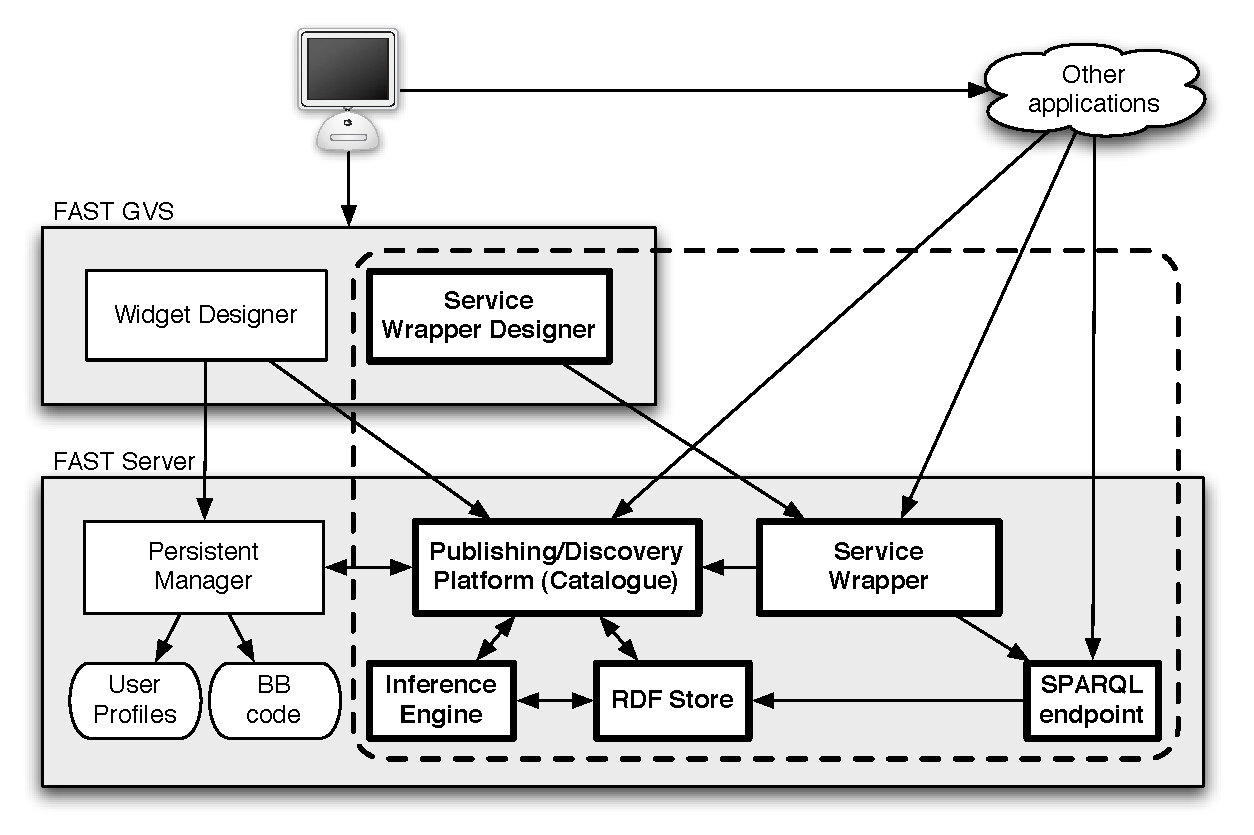
\includegraphics[width=\linewidth]{images/fast_architecture.pdf}
    \caption{Overview of the FAST architecture}
    \label{fig:fast_architecture}
  \end{center}
\end{figure}

In order to provide a better understanding of these components, we describe a number of concepts related to FAST in this section. 
A \emph{gadget} is the end product of the platform, ready to be run in any ordinary web browser, usually through a mashup platform. 
An undeployed gadget is also called \emph{screenflow}, which comprises a set of \emph{screens} connected through their \emph{pre-} and \emph{post-conditions}. A screen is the most complex building block fully functional by itself,
visually similar to a tab in a tabbed application.
It is composed by a \emph{form} conveying the graphical interface, and a set of \emph{operators} and \emph{back-end services}, wrapped into so-called \emph{service resources}.

The publishing platform, also called \emph{catalogue}, covers several important purposes, such as storage, indexing, publication and search of gadgets, gadget building blocks and user profiles.
% , as well as some level of ontology mediation to facilitate the integration of services from different parties (first steps in this direction are outlined in \cite{Ambrus:2009it}).
The service wrapper tool is used to create wrappers for third-party web services, transforming them into building blocks to be stored and reused within the FAST platform.


%!TEX root = paper.tex

\section{Conclusions and future work}
\label{sec:conclusions}

It has been demonstrated that adopting web services standards lead enterprises to increase operational efficiency, reduce costs and strengthen the relations with partners. Many of these standards have been widely adopted, such as WSDL, XML and UDDI, and many companies offer access to their information and operational systems through web services. 
However, when dealing with end-users, the process for publication and consumption is not well defined. 
The common way of publishing services is by providing some sort of definition on their websites, such a WSDL document and further details in a human-readable HTML page. 
Discovery is performed through a search engine or aggregator, mainly in a syntax-based way. For consumption, in most cases, consultants with good programming skills are required. 
In a move towards improving this situation, the work presented in this paper empowers the end-user with a platform (the \emph{catalogue}) to easily discover services based on functional behaviour (pre-/post-conditions) and other metadata, being able to download a so-called resource adapter allowing the consumption of web services using standard languages to execute within a web browser, and a tool to transform, in an interactive manner, formal definitions of web services into these resource adapters, ready for being publisher into the catalogue.

The current version of the wrapping tool permits to create resource adapters for RESTful web services. 
As a next step, we will tackle SOAP-based web services described in WSDL documents. Once this is done, we will cover the two major paradigms for defining web service interfaces. However, we also consider to include semantically enriched WSDL documents using SAWSDL, and to support other SWS approaches such as WSMO-lite services. 

Another limitation of the platform is inherent in web client technologies and the cross-domain policy for security. This is solved within FAST using platform-dependent API calls. Hence, the code generated makes use of the FAST API, which will be transformed depending on the mashup platform the user intends to deploy the gadget. To avoid these issues, and to be able to provide platform-independent code right away, we are planning to deploy the JSONRequest approach as proposed by \cite{crockford2006} and other solutions.



\subsubsection*{Acknowledgments.} This work is supported in part by the European Commission under the first call of its Seventh Framework Program (FAST STREP Project, grant INFSO-ICT-216048) and in part by Science Foundation Ireland under Grant No. SFI/08/CE/I1380 (L\'ion-2).


\bibliographystyle{apalike}
\bibliography{paper}


\section*{Checklist of Items to be Sent to Volume Editors}
Here is a checklist of everything the volume editor requires from you:


\begin{itemize}
\settowidth{\leftmargin}{{\Large$\square$}}\advance\leftmargin\labelsep
\itemsep8pt\relax
\renewcommand\labelitemi{{\lower1.5pt\hbox{\Large$\square$}}}

\item The final \LaTeX{} source files
\item A final PDF file
\item A copyright form, signed by one author on behalf of all of the
authors of the paper.
\item A readme giving the name and email address of the
corresponding author.
\end{itemize}
\end{document}
